\documentclass[a4paper,11pt]{article}
\usepackage{fullpage}
\usepackage{hyperref}
\usepackage{url}
\usepackage{graphicx}

\title{'Awesome Game' Report}
\author{Rafal Szymanski, Maciej Albin, Suhaib Sarmad, Maciej Albin}


\begin{document} 
	\maketitle
	
	\tableofcontents
	\newpage
	
	\section{Introduction}
	
		The purpose of this assignment was to create a networked application with a game element in it. We found the project quite open ended, and after consultation with the project coordinator, we were told we do not have to use any technologies provided by the Department of Computing, but can use our own, as long as the final product works and is presentable.

		Because of this, we decided to take a very novel approach, and use very new technologies that are still in active development, but are nevertheless incredibly interesting. Our game/project does not utilize the departments database servers or Apache/Tomcat servers. We decided to deploy the project on our own VPS server.

		We have had a number of problems using our chosen technologies due to the fact how new they are and the fact that bug fixes are pretty much released every day. Nevertheless, we have managed to create a usable and playable game using client side technologies such as the HTML5 canvas, JS, and websockets, and server side technologies that include Node.Js, MongoDB, and websockets.
	
		
	\section{Game Idea and Mechanics}
	
		Our game takes place in space, on a two dimensional grid visible from above. Here is a screenshot of our game to support the explanation of rules that follows in this report.
		
		\begin{figure}[htb]
		\begin{center}
		\leavevmode
		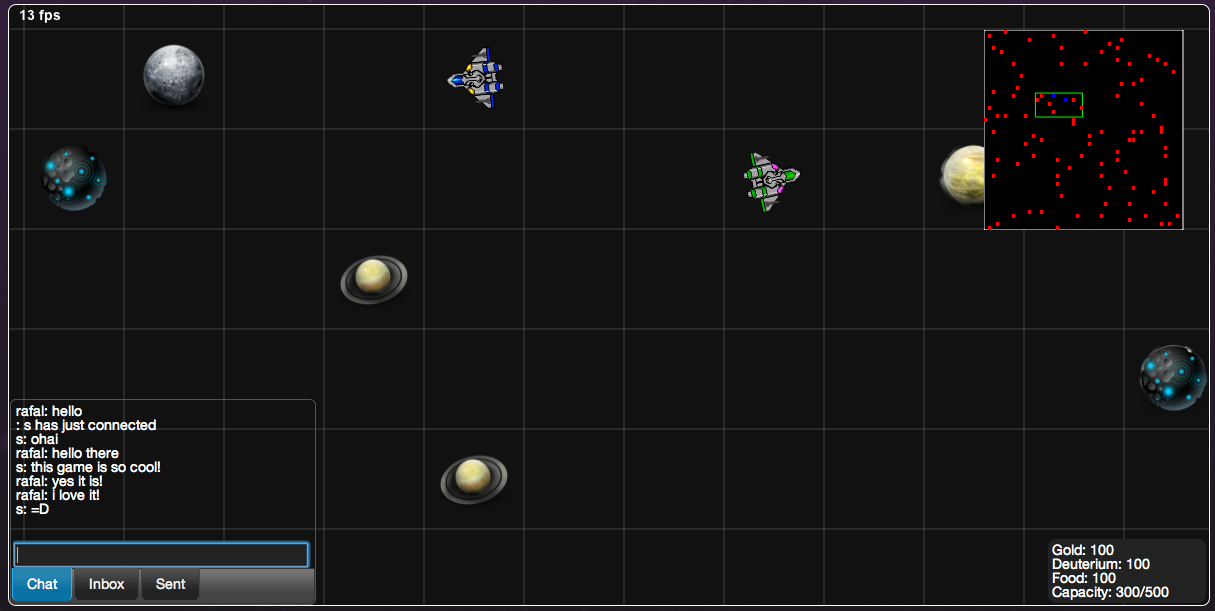
\includegraphics[scale=0.35]{screen1.png}
		\end{center}
		\caption{Ingame Screenshot}
		\label{fig:ingame1}
		\end{figure}
	
		\subsection{Game Rules}
		
			We have Players who own spaceships and travel from Planet to Planet, by clicking on their ship, and then selecting a board position to move to. When that is done, the player's ship is animated towards its new destination.
		
			After registering at the registration screen (username, password, email), each user starts out with a certain amount of each resource. The resources in our game include Gold, Food, and Deuterium. Each player starts out with 100 of each resource. Additionally, a player's ship has a capacity so that at any one time he cannot carry more resources than his capacity. One can buy a capacity upgrade when one has enough resources.
		
			The universe also consists of planets, each of which has resources, a type (Agricultural, Mining, or Factory), a size (Dwarf, Terrestrial, or Giant), and an exchange rate. Planets that produce a certain resource sell it for less. Every minute the prices get updated according to our algorithm. Also, every 5 minutes, planets produce resources.
		
			The objective is for Players to travel around from Planet to Planet, and to trade resources to their advantage, ie to end up with the largest amount of resources. Whenever a player arrives at a grid square that has a planet in it, the trade screen pops up and the player can decide what to trade based on a barter system. The player has to select which resource he/she wants to buy from the planet, and which resource he wants it trade it for. He can then do the trade, leave the trade screen, and keep on travelling around the universe. The game is currently open ended, and there is no finish. Our goal at the beginning was to have a larger amount of features such as owning multiple ships, owning a specific planet, or having fights with other ships, but we did not have the time to implement this.
			
			Additionally, travelling uses up Deuterium, which is used as fuel. In the current version, the user must be careful not to run out of deuterium in the middle of space, or he will not be able to move and do anything. In a future version, we plan to add inter-ship trading, so that two ships can trade together in case one runs out of fuel.
			
		
		\subsection{Minimap}
			
			As part of our game, and our quest to make it feel/look like an RTS game, we have created a minimap in the top right corner. The minimap shows the position of all planets in one color, along with all players shown in a different color. The minimap is synchronised in real time. One of our ideas was to implement a fog of war, but we did not have the time to do this.
			
			Here is a screenshot of the minimap:
			
			\begin{figure}[htb]
			\begin{center}
			\leavevmode
			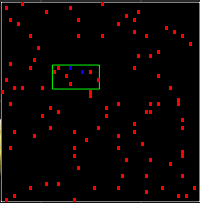
\includegraphics[scale=0.7]{minimap.png}
			\end{center}
			\caption{Minimap}
			\label{fig:minimap}
			\end{figure}
			
			
		\subsection{Chat}
			
			We have also implemented a simple chat application. Upon login, the chat application is at all times present in the bottom left corner of the game. Players can type chat messages, and upon submitting the message, the message is distributed and shown to all clients currently connected to the server and playing the game. Additionally, this chat box also informs players of other people who have just logged in, or that have disconnected.
			
		\subsection{Map Editor and Generator}
		
		The map editor, as the name indicates, is a tool which allows an administrator to create or edit a universe in which players move around and interact. The editor, due to it's interactive nature, uses the same front-end technologies as the game itself. For consistency, we use EaselJS for handling the HTML5 canvas and JQuery for certain inputs and advanced functions.

		Thanks to the efficient way we structured our game, we were able to reuse resources such as the Map, Planet and Minimap elements as well as stylesheets, all of which which helped keep things consistant and made debugging easier.
		
		\begin{figure}[htb]
		\begin{center}
		\leavevmode
		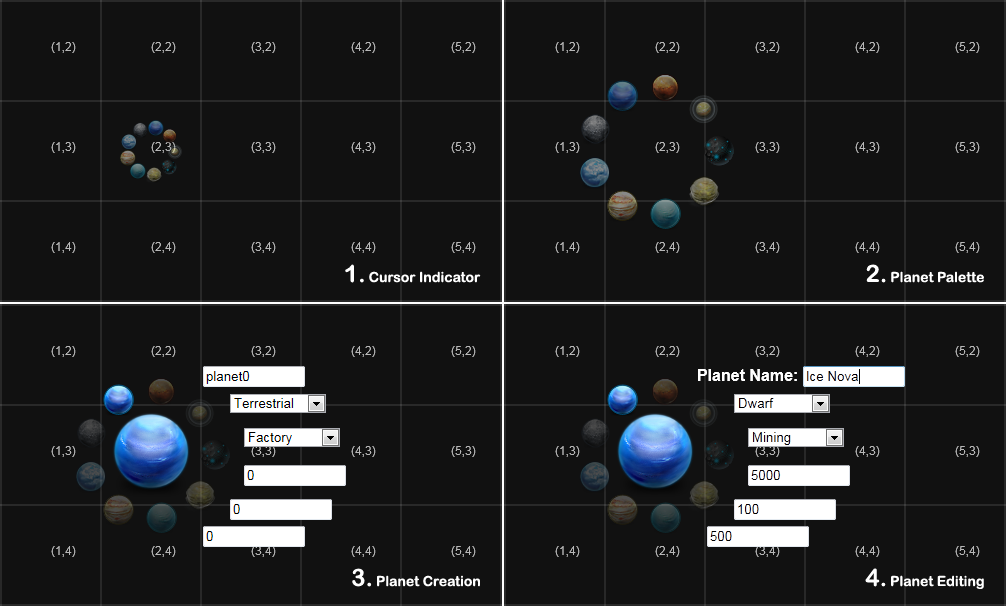
\includegraphics[scale=0.6]{mapedit.png}
		\end{center}
		\caption{Map Editor}
		\label{fig:mapedit}
		\end{figure}

		A lot of effort went into making the map editor comprehensive and easy to use. Once the page has loaded, the administrator has a "Planet Palette" available to him which follows his cursor location. On clicking on an empty grid position, the palette expands, allowing the selection of a planet image to use for creating a new planet. Once a planet has been created, the planet's general information can be editted using the convenient text boxes that appear next to the planet. Focussing a particular text box pushes a description of the selected field. This allows for a clean looking interface which stays functional and conveys all necessary information as needed. Deleting a planet is done by clearing the planet's name and saving its information (clicking on the planet once again).

		As well as individual planet creating and editing capabilities, the map edit also allows for generating entire maps procedurally. The administrator just has to specify the number of planets to be generated and the min/max resources a planet can have. Planet names are selected from a list of actual planets; this is a small example of how games employ tangential learning to educate their players without them necessarily knowing.

		Once a map is ready, it can be exported and applied to the server's database. We use JQuery to send the map to the server which then applies the new map to the game.

		Development of the map editor showed us the importance of using in-house-made tools in certain situations, as well as making sure said tools are easy to use. Although visual appeal is not as important in an in-house-used tool as it is in the actual game, it does help to make tools pretty as it is more pleasant to use a good looking tool than a tool which is hard to look at.
		
		\subsection{Messaging System}
		We have created a messaging system for the site so that players can send each other private messages.

		Our initial design was to have the inbox as a seperate page from the game, but as we started development we realised that it would be better to include it as part of the main page and hence chose the design of the messaging centre as a dialog box that comes up when playing the game.
		The dialog box was implemented with the help of the jQuery javascript library.

		When the dialog box is called then the list of messages that the user has are loaded. This is done by invoking a get request to the server which then queries our database to retrive the messages. Careful consideration had to be taken here as not all of the message content is loaded, only the essential "header" information (i.e. who the message is from and whether it has been read).

		When the user wants to select a particular message then they click on it and in turn the content of the message is retrieved using a post request with the unique identifier of the message. The unique identifier is used to retrieve the message content from our database and returns it to the client. The message is also marked as 'read' at this point.

		As far as rendering the message content is concerned, we only had one place to do this, so manipulation of the Document Object Model (DOM) was required, and again this was done using jQuery, which dynamically changed the message being selected and also changed the message content of the current message being selected.

		In addition to this we also created a real time notification service, so that if a user recieves a message whilst playing the game then they get a notification on the game canvas that they recieved a message.
		
		
	
	\section{Client Side Technologies}
		On the client side, we employ Javascript and the HTML5 canvas along with a library, EaselJS, that makes drawing on the HTML5 canvas a bit less painful. Nevertheless, using the HTML5 canvas is a quite tedious process.
	
		\subsection{HTML5 Canvas}
			Since it's quite new and cool addition to HTML, we decided to play around with, and implement our game, using the HTML5 canvas element. By itself, the HTML5 canvas is not particularly developer-friendly for doing animations due to the fact that it uses a immediate rendering mode, meaning you have to clear the canvas before drawing a new frame. Additionally, creating a large map with scrolling abilities seemed to be quite difficult, which is why we decided to use a wrapper API around the HTML5 canvas, EaselJS, which provides for a quite easy way to animate things on the HTML5 canvas.
			
		\subsection{EaselJs}
			EaselJs\footnote{\url{http://easeljs.com}} is wrapper around the canvas element that greatly simplifies animation. It has proved to be quite easy to use, but we have found it very difficult to properly use it, as in our game uses up a lot of CPU cycles, and tends to run only at 20FPS even on good computers. 
			
			While hand-coding the graphics and animations in HTML5 would have most likely provided for a much higher rendering speed, we didn't find it worthy to spend so much time doing HTML5 animations by hand, and decided to concentrate more on creating a robust server back-end.
					
	\section{Server Side Technologies}
		On the server side we are using a number of new and rather untested technologies, such as the asynchronous evented IO framework Node.js\footnote{\url{http://nodejs.org}} written in javascript, socket.io\footnote{\url{http://socket.io/}} to do client/server communication, and MongoDB\footnote{\url{http://www.mongodb.org/}} together with the Mongoose ORM\footnote{\url{http://mongoosejs.com/}}  for Node for storage of data.
	
		\subsection{Node.js}
		
			Node.js provides asynchronous evented IO. The node process is itself a single thread, and it does not spawn more threads to handle more clients, unlike other servers such as Apache. Me and my team found this to be quite cool, and decided to learn Node.js, and implement our game using this technology.
			
			On the whole, it is very cool and exciting, and we will probably use it in the future for other projects.
			
			One problem/inconvenience with using this type of asynchronous event based server, and the fact that it's written in Javascript, is that that many times you have many nested callback functions that are to be executed when the parent function finishes. Due to this, writing code that interacts with the database is not particularly easy, since you have to care about the asynchronous nature, and pass callbacks. This is unlike in languages such as PHP, where if in line x you execute a database query and assign the result to some variable, you are expecting that variable to be available in the next line due to the threaded and blocking nature of Apache/PHP. This is not the case in Node.js, which took some time getting used to.
			
			Nevertheless, Node.js is a very exciting project, and we are very glad we have decided to learn and use it.		
		
		\subsection{Socket.IO}
		
			Socket.IO is the library we use both on the client and server side, in order to communicate data between the client the server. Socket.IO is very neat due to the fact that it has many fallbacks in order to accommodate older browsers which don't support the newest standard in client/server communications, Websockets. In case Websockets are not available in the browser being used, socket.io will fallback to other technologies such as ajax polling.
		
			We communicate over socket.io for pretty much all the information we need, such as sending animation initialization packets, handling the chat, or getting trading information.
		
		\subsection{Data Storage using MongoDB}
			At first, we were using MySQL, then switched to PostgreSQL, but we didn't like the Node libraries available to handle both MySQL and PostgreSQL, so we decided to use something different.
			 
			Since we have never had any experience using NoSQL data storage solutions, we decided now it's the time to try one out, and we settled on MongoDB.
			
			Node.js has an ORM for MongoDB called Mongoose, which we used extensively throughout the project. With it, we can define models, such as a User model:
			
			\begin{verbatim}
var UserSchema = new Schema({
  username: {type: String, unique: true},
  password: String,
  email: String,
  joined: {type: Date, default: Date.now},
  admin: {type: Boolean, default: false},
  position: {
    x: {type: Number, default: 3},
    y: {type: Number, default: 3}
  },
  rotation: {type: Number, default: 0},
  shipType: {type: Number, default: 1},
  resources: resources,
  capacity: {type: Number, min: 0, default: 500}
});
			\end{verbatim}
		
			Then, we can use this model to get back data about the user, or write data back to the Mongo store.
			A consideration is that MongoDB should always be ran with a secondary DB server in order for backup, but we are running it only on one server due to the fact we don't have more than one server.
			
	
	\section{Libraries and Content Used}
		In this section, we acknowledge the content (ship and planet images) we used, and the Libraries and software that we used.
		
		\subsection{Content Used}
			\begin{itemize}
				\item Planet images taken from here\footnote{\url{http://icones.pro/en/internet-network-connections-planet-png-image.html}} and here\footnote{\url{http://www.softicons.com/free-icons/object-icons/solar-system-icons-by-parthiban-mohanraj}}
				\item Ship images from WHEREWOIRHWEHRHWER
				\item The site background was created by us in Photoshop
			\end{itemize}
			
		\subsection{Libraries and Software Used}
			\begin{itemize}
				\item Node.js \url{http://nodejs.org}
				\item npm \url{http://npmjs.org}
				\item EaselJS \url{http://easeljs.com}
				\item jQuery \url{http://jquery.com/}
				\item node bcrypt module \url{https://github.com/jonmaim/node.bcrypt.js}
				\item node connect module \url{https://github.com/senchalabs/Connect}
				\item express.js framework \url{http://expressjs.com/}
				\item node forms module \url{https://github.com/caolan/forms}
				\item jade templating language \url{http://jade-lang.com/}
				\item mongoose ORM \url{http://mongoosejs.com/}
				\item MongoDB \url{http://www.mongodb.org/}
				\item socket.io \url{http://socket.io/}
				\item underscore.js \url{http://documentcloud.github.com/underscore/}
				\item nodemailer module \url{http://www.nodemailer.org/}
			\end{itemize}
	
	\section{Conclusion}
	
	Overall, we are quite happy with the result of our project. We have managed to learn many new technologies, since no one from the group has ever used any of the technologies we decided to use, so we are finishing the project with a good knowledge of Javascript, Node.JS, MongoDB, and HTML5 canvas.
	
	We are very fond of the networking aspect of our game, since this is the first real time networked application that we have written. As soon as someone connects/disconnects/moves, the change is propagate by the server to all the clients, and we have a real-time looking game. 
	
	We seem to have a slight problem with synchronising movement animations because different people run the game at different frame rates, but we are currently working on a way to fix this.
	
	We didn't have the time to implement all the features that we wanted, such as inter-ship trading. Another aspect we are not that happy about is the performance of the graphics in the canvas. The rendering is very slow, peaking at around 20 FPS even on quite good and recent computers. This comes most likely from our misunderstanding of how to properly use the EaselJS library, but even after communicating on the EaselJS group, we didn't seem to be able to optimize the rendering.
	
	
	
\end{document}